\documentclass{article}
\usepackage{graphicx}
\usepackage{paralist} % needed for compact lists
\usepackage[normalem]{ulem} % needed by strike
\usepackage[urlcolor=blue,colorlinks=true]{hyperref}
\usepackage[utf8]{inputenc}  % char encoding
\usepackage{site.css}  % user defined

\title{La Vie en TSI}
\begin{document}
\date{CPGE TSI Troyes}
\maketitle
\clearpage

<IMG ALIGN="middle" SRC="img/banniere-velo.jpg" BORDER="0">
<div id="nav">

\begin{itemize}
\item \htmladdnormallink{Accueil}{index.html}
\item \htmladdnormallink{Devenir Ingénieur(e)}{devenirIngenieur.html}
\item \htmladdnormallink{Formation}{formation.html}
\item \htmladdnormallink{Hébergement}{internat.html}
\item \htmladdnormallink{Témoignages \& Résultats}{resultats.html}
\item \htmladdnormallink{La vie en TSI}{laVie.html}
</div>

<DIV id="sidebar">

\end{itemize}

\subsubsection*{Nous Contacter}

\begin{compactitem}
\item \htmladdnormallink{Venir au Lycée}{plan.html}
<li>
<script language="javascript">
<!--
var pomme = "cpgetsi.lombards";
var poire = "free.fr?subject=[site]";
var peche = "Nous contacter";
document.write('<a href="mai' + 'lto:' + pomme + '@' + poire + '">');
document.write(peche + '</a>');
// -->
</script>
\end{compactitem}

\subsubsection*{S'inscrire en CPGE}

\begin{compactitem}
\item \htmladdnormallink{La procédure}{Inscription.html}
\item \htmladdnormallink{Le site Admission Post-bac}{http://www.admission-postbac.fr}
\item \htmladdnormallink{Le guide du candidat}{http://www.admission-postbac.fr/site/guide\_2012/Guide\_du\_candidat\_2012-20-01-2012.pdf}
\end{compactitem}

\subsubsection*{En prépa à Troyes}

\begin{compactitem}
\item \htmladdnormallink{Le site des Prépas Troyennes}{http://web.prepatroyes.org}
\item \htmladdnormallink{Plaquette de présentation}{http://web.prepatroyes.org/files/plaquettes/PREPA\%202012\%20BAT\%201.pdf}
\end{compactitem}

</DIV>
<DIV id="Contenu">

\section*{Le tour de Troyes}

Les élèves et les profs de toutes les classes prépa de Troyes participent ensembles au Tour du Bouchon, un marathon dans le centre de la ville de Troyes.

 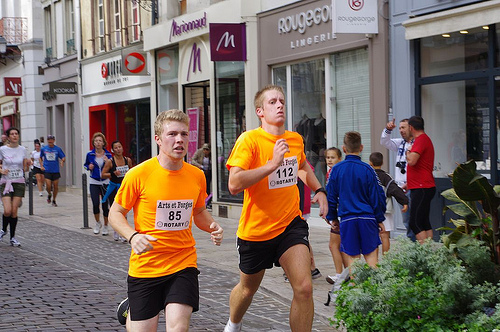
\includegraphics{img/max-PA.jpg} 

\begin{center}\begin{tabular}{l}
Maxence et PA \\
\end{tabular}\end{center}

 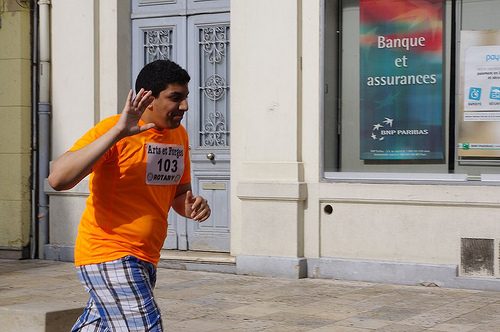
\includegraphics{img/Farid.jpg} 

\begin{center}\begin{tabular}{l}
Farid \\
\end{tabular}\end{center}

\section*{Le Ski}

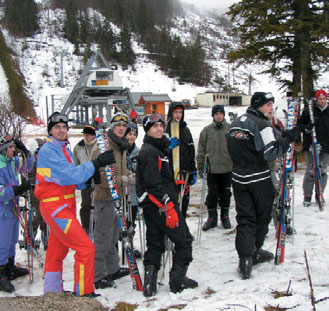
\includegraphics{img/ski.png} 
Les 2013-2014 verront le retour d'une des traditions de la TSI : le voyage au ski organisé par les professeurs au retour des vacances de fin d'année.

</div></div><div id="footer">
    <script type="text/javascript" language="javascript"><!--
eval(unescape(
'%76%61%72%20%61%3D%27%70%63%65%67%73%74%2E%69%6F%6C%62'+
'%6D%72%61%73%64%66%40%65%72%2E%65%72%66%27%3B%76%61%72'+
'%20%64%3D%22%22%3B%20%76%61%72%20%62%3D%27%27%3B%66%6F'+
'%72%28%76%61%72%20%63%3D%30%3B%63%3C%61%2E%6C%65%6E%67'+
'%74%68%3B%63%2B%2B%2C%63%2B%2B%29%7B%62%3D%62%2B%61%2E'+
'%73%75%62%73%74%72%69%6E%67%28%63%2B%31%2C%63%2B%32%29'+
'%2B%61%2E%73%75%62%73%74%72%69%6E%67%28%63%2C%63%2B%31'+
'%29%7D%64%6F%63%75%6D%65%6E%74%2E%77%72%69%74%65%28%27'+
'%3C%61%20%68%72%65%66%3D%22%6D%61%69%6C%74%6F%3A%27%2B'+
'%62%2B%64%2B%27%22%20%74%69%74%6C%65%3D%22%27%2B%62%2B'+
'%27%22%3E%43%6F%6E%74%61%63%74%65%72%20%6C%65%20%77%65'+
'%62%6D%61%73%74%65%72%20%64%75%20%73%69%74%65%3C%2F%61'+
'%3E%27%29')); // -->
</script>

novembre 2013

</div><div id="fake">

% LaTeX2e code generated by txt2tags 2.6 (http://txt2tags.org)
% cmdline: txt2tags -t tex laVie.t2t
\end{document}
